\documentclass[pre,twocolumn,english,longbibliography]{revtex4} %twocolumn,

%\usepackage[latin9]{inputenc}
\setcounter{secnumdepth}{3}
\usepackage{babel}
\usepackage{amsmath}
\usepackage{amssymb}
\usepackage{graphicx} 
\usepackage{epstopdf} %add for pdflatex, nut don^{\prime}t compile because of invisible character copied from .bbl file?
\usepackage[T1]{fontenc}
\usepackage[utf8x]{inputenc} 
\usepackage{esint}
\usepackage{verbatim}
%\usepackage[hyphens]{url}
\usepackage[unicode=true]{hyperref}
\usepackage[capitalize,nameinlink]{cleveref}
\creflabelformat{equation}{#2\textup{#1}#3}
\usepackage[table]{xcolor}
\newcommand{\re}[1]{\textcolor{magenta}{#1}}
%\loadpackage{url}
%\usepackage[unicode=true]{hyperref}
%\setcounter{biburllcpenalty}{7000}
%\setcounter{biburlucpenalty}{8000}
%\usepackage{breakurl}
%\hypersetup{breaklinks=true}
%\usepackage[hyperref,eprint=false]{biblatex}
\makeatletter

%%%%%%%%%%%%%%%%%%%%%%%%%%%%%% LyX specific LaTeX commands.
\pdfpageheight\paperheight
\pdfpagewidth\paperwidth

%%%%%%%%%%%%%%%%%%%%%%%%%%%%%% User specified LaTeX commands.
\usepackage{bbold}
\newcommand{\overbar}[1]{\mkern 1.5mu\overline{\mkern-1.5mu#1\mkern-1.5mu}\mkern 1.5mu}
\usepackage{xcolor}
\hypersetup{
    colorlinks,
    linkcolor={red!50!black},
    citecolor={blue!50!black},
    urlcolor={blue!80!black}
}

\usepackage{amsmath}
\DeclareMathOperator*{\argmax}{argmax}
\DeclareMathOperator*{\argmin}{argmin}

\newcommand{\beginsupplement}{%
        \setcounter{table}{0}
        \renewcommand{\thetable}{S\arabic{table}}%
        \setcounter{figure}{0}
        \renewcommand{\thefigure}{S\arabic{figure}}%
     }

\newcommand{\beqn}{\begin{eqnarray}}
\newcommand{\eeqn}{\end{eqnarray}}
\newcommand{\beq}{\begin{equation}}
\newcommand{\eeq}{\end{equation}}
\newcommand{\av}[1]{\langle{#1}\rangle{}}
\newcommand{\abs}[1]{|#1|}
\newcommand{\<}{\langle}
\renewcommand{\>}{\rangle}
\newcommand{\AW}[1]{{\color[rgb]{0,0,1}#1}}
     
\makeatother

\begin{document}

\title{Inferring the immune response from repertoire sequencing}

\author{Maximilian Puelma Touzel}
%\email[]{puelma@lpt.ens.fr}

\affiliation{Laboratoire de physique de l'\'Ecole normale sup\'erieure
  (PSL University), CNRS, Sorbonne  Universit\'e, Universit\'e de
  Paris, 75005 Paris, France}
\affiliation{Mila, Université de Montréal, Montreal, Canada}

\author{Aleksandra M. Walczak}
\thanks{Corresponding authors. These authors contributed equally.}
\affiliation{Laboratoire de physique de l'\'Ecole normale sup\'erieure
  (PSL University), CNRS, Sorbonne  Universit\'e, Universit\'e de
  Paris, 75005 Paris, France}

\author{Thierry Mora}
\thanks{Corresponding authors. These authors contributed equally.}
\affiliation{Laboratoire de physique de l'\'Ecole normale sup\'erieure
  (PSL University), CNRS, Sorbonne  Universit\'e, Universit\'e de
  Paris, 75005 Paris, France}

\vspace{0.5cm}

\begin{abstract}
  High-throughput sequencing of B- and T-cell receptors makes it possible to track immune repertoires across time, in different tissues, and in acute and chronic diseases or in healthy individuals. However, quantitative comparison between repertoires is confounded by variability in the read count of each receptor clonotype due to sampling, library preparation, and expression noise. Here, we present a general Bayesian approach to disentangle repertoire variations from these stochastic effects. Using replicate experiments, we first show how to learn the natural variability of read counts by inferring the distributions of clone sizes as well as an explicit noise model relating true frequencies of clones to their read count. We then use that null model as a baseline to infer a model of clonal expansion from two repertoire time points taken before and after an immune challenge. Applying our approach to yellow fever vaccination as a model of acute infection in humans, we identify candidate clones participating in the response.

%\re{Good, but need to add new, main takeaways.} High-throughput sequencing provides access to expression-level detail of cell populations. Identifying signal in this data is nevertheless a challenge: intrinsic variability, vast sub-sampling, and indirect access together make difficult the reliable and accurate inference of the changes in population size due to environmental perturbations. Here, in the context of antigen-perturbed immune cell repertoires, we formulate access to the unobserved repertoire using a generative model of observed sequence count pairs from a reference and differentially-expressed condition. When applied to pairs of replicates, our model captures the natural variability in the system, giving reproducible behavior across donors and, in spite of sub-sampling, provides plausible parameter estimates for the underlying repertoire. Using this replicate model as a baseline, we then formulate the differentially expressed condition using a prior distribution on the ratio of a clone’s frequency pair for pairs of repertoires sampled at different time points. The posterior distribution of this ratio for each observed clone is then obtained and used to characterize if and how strongly it participates in the response. Applying our approach to yellow fever vaccination as a model of acute infection in humans, we identify candidate clones participating in the response.   

\end{abstract}

\maketitle

Next generation sequencing allows us to gain access to repertoire-wide data supporting more comprehensive repertoire analysis and more robust vaccine design \citep{Benichou2011}. 
Despite large-scale efforts\citep{Glanville2017}, how repertoire statistics respond to such acute perturbations is unknown. 
Longitudinal repertoire sequencing (RepSeq) makes possible the characterization of repertoire dynamics. 
Despite the large number of samples (clones) in these datasets lending it to model-based inference, there are few existing model-based approaches to this analysis. 
Most current approaches (e.g. \citep{Chu2019}) quantify repertoire response properties using measurement statistics that are limited to what is observed in the sample, rather than what transpires in the individual.
Model-based approaches, in contrast, can in principle capture features of the actual repertoire response to, for instance ongoing, natural stimuli, modeled as a point process of infections, and giving rise to diffusion-like response dynamics. 
Another regime for model-based approaches is the response to a single, strong perturbation, such as a vaccine, giving rise to a stereotyped, transient response dynamics.
In either case, a measurement model is needed since what is observed (molecule counts) is indirect.
We also only observe a small fraction of the total number of clones, so some extrapolation is necessary. 
Finally, both the underlying clonal population dynamics and the transformation applied by the measurement is stochastic, each contributing its own variability, making inferences based on sample ratios of molecule counts inaccurate.

Inference of frequency variation from sequencing data has been intensely researched in other areas of systems biology, such as in RNAseq studies. There, approaches are becoming standardized (DESEQ2 \citep{Love2014},EdgeR \citep{Robinson2008}, etc.) and technical problems have been formulated and partly addressed.
The differences between RNAseq and RepSeq data, however, means that direct translation of these methods is questionable. Moreover, the known structure of clonal populations may be leveraged for model-based inference using RepSeq, potentially providing advantages over existing RNAseq-based approaches.

Here, we take a generative modeling approach to repertoire dynamics. Our model incorporates known features of clonal frequency statistics and the statistics of the sequencing process. The models we consider are designed to be learnable using RepSeq data, and then used to infer properties of the repertoires of the individuals providing the samples. To guide its development, we have analyzed a longitudinal dataset around yellow fever vaccination (some results of this analysis are published \citep{Pogorelyy12704}). Yellow fever serves as model of acute infection in humans and here we present analyses of this data set that highlights the inferential power of our approach to uncover perturbed repertoire dynamics. 



\section*{Results}

\subsection*{Modeling repertoire variation}

To describe the stochastic dynamics of an individual clone, we define a probabilistic rule relating its frequency $f'$ at time $t'$ to its frequency $f$ at an earlier time $t$: $G(f',t'|f,t)$. In this paper, $t$ and $t'$ will be pre- and post-vaccination time points, but more general cases may be considered.
It is also useful to define the probability distribution for the clone frequency at time $t$, $\rho(f)$ (Fig.~\ref{fig:fullmodel}A).

The true frequencies of clones are not directly accessible experimentally. Instead, sequencing experiments give us number of reads for each clonotypes, $n$, which is a noisy function of the true frequency $f$, described by the conditional probability $P(n|f)$ (Fig.~\ref{fig:fullmodel}B). Correcting for this noise to uncover the dynamics of clones is essential and is a central focus of this paper.

Our method proceeds in two inference steps, followed by a prediction step. First, using same-day replicates at time $t$, we jointly learn the characteristics of the frequency distribution $\rho(f)$  (Fig.~\ref{fig:fullmodel}A) and the noise model $P(n|f)$ (Fig.~\ref{fig:fullmodel}B). Second, by comparing repertoires between two time points $t$ and $t'$, we infer the parameters of the evolution operator $G(f',t'|f,t)$, using the noise model and frequency distribution learned in the first step (Fig.~\ref{fig:fullmodel}C). Once these two inferences have been performed, the dynamics of individual clones can be estimated by Bayesian posterior inference. These steps are described in the remaining Results sections. In the rest of this section, we define and motivate the classes of model that we chose to parametrize the three building blocks of the model, schematized in Fig.~\ref{fig:fullmodel}: the clone size distribution $\rho(f)$, the noise model $P(n|f)$, and the dynamical model $G(f',t'|f,t)$.

\begin{figure*}
\includegraphics[width=\textwidth]{Fig1_model}
\centering{}
\caption{
\emph{Model components}. (A) Clone frequencies are sampled from a prior density of power law form with power $\nu$ and minimum frequency, $f_\textrm{min}$. (B) Each clone's frequency $f$ determines the count distribution, $P(n|f)$, that governs its mRNA count statistics in the observed sample. We consider 3 forms for $P(n|f)$: Poisson, negative binomial, and a two-step (negative binomial to Poisson) model. The negative binomial and two-step measurement models are parametrized through a mean-variance relationship specifying the power, $\gamma$, and coefficient, $a$, of the over-dispersion of cell count statistics. The mean cell count scales with the number of cells in the sample, $M$, while the mean read count scales with with the number of cells, $m$, and the sampling efficiency, $M/N_{\textrm{read}}$, with $N_{\textrm{read}}$ the measured number of molecules in the sample. The parameters of the measurement model are learned on pairs of sequenced repertoire replicates.  (C) Differential expression is implemented in the model via a random log fold change, $s$, distributed according to the prior $\rho(s|\theta_\textrm{exp})$. The prior's parameters, $\theta_\textrm{exp}$, are learned from the dataset using maximum likelihood. Once learned, the model is used to compute posteriors over $s$ given observed count pairs, which is used to make inferences about specific clones.
\label{fig:fullmodel}}
\end{figure*}

\subsubsection*{Distribution of lymphocyte clone sizes}

The distribution of clone sizes in memory or unfractioned TCR repertoires has been observed to follow a power law in human \cite{Mora2016e,Gerritsen_thesis,Greef2019} and mice \cite{Zarnitsyna2013,Heather2017}. These observations justify parametrizing the clone size distribution as
\beq
\rho(f)=Cf^{-\nu}, \qquad f_{\rm min}\leq f<1,
\eeq
and $C$ a normalizing constant. 
We will verify in the next section that this form of clone size distribution describes the data well.
For $\nu>1$, which is the case for actual data, the minimum $f_{\rm min}$ is required to avoid the divergence at $f=0$. This bound also reflects the smallest possible clonal frequencies given by the inverse of the total number of lymphocytes, $1/N_{\rm cell}$. The frequencies of different clones are not independent, as they must sum up to 1: $\sum_{i=1}^Nf_i=1$, where $N$ is the total number of clones in the organism. The joint distribution of frequencies thus reads:
\beq
\rho_N(f_1,\ldots,f_N)\propto\prod_{i=1}^N\rho(f_i)\delta\left(\sum_{i=1}^Nf_i-1\right).
\eeq
This condition, $\sum_{i=1}^Nf_i=1$, will be typically satisfied for large $N$ as long as $\<f\>=\int \textrm{d}f \,f\rho(f) = 1/N$ (see Methods), but we will need to enforce it explicitly during the inference procedure. 

\subsubsection*{Noise model for sampling and sequencing}

The noise model captures the variability in the number of sequenced reads as a function of the true frequency of its clonotypes in the considered repertoire or subrepertoire. The simplest and lowest-dispersion noise model assumes random sampling of reads from the distribution of clonotypes. This results in $P(n|f)$ being given by a Poisson distribution of mean $fN_{\rm read}$, where $N_{\rm read}$ is the total number of sequence reads. Note that for the data analyzed in this paper, reads are collapsed by unique barcodes corresponding to individual mRNA molecules. 

Variability in mRNA expression as well as library preparation introduces uncertainty that is far larger than predicted by the Poisson distribution. This motivated us to model the variability in read counts by a negative binomial of mean $\bar n=fN_{\rm read}$ and variance $\bar n+a\bar n^\gamma$, where $a$ and $\gamma$ control the over-dispersion of the noise. Negative binomial distributions were chosen because they allow us to control the mean and variance independently, and reduce to Poisson when $a=0$. These distributions are also popular choices for modeling RNAseq variability in differential expression methods \cite{Robinson2010,Love2014}.

A third noise model was considered to account explicitly for the number of cells representing the clone in the sample, $m$. In this two-step model, $P(m|f)$ is given by a negative binomial distribution of mean $\bar m=fM$ and variance $\bar m+a\bar m^\gamma$, where $M$ is the total number of cells represented in the sample. $P(n|m)$ is a Poisson distribution of mean $mN_{\rm read}/M$. The resulting noise model is then given by $P(n|f)=\sum_m P(n|m)P(m|f)$. The number of sampled cells, $M$, is unknown and is a parameter of the model. Note that this two-step process with the number of cells as an intermediate variable is specific to repertoire sequencing, and has no equivalent in RNAseq differential expression analysis.

\subsubsection*{Dynamical model of the immune response}
Finally, we must specify the dynamical model for the clonal frequencies. In the context of vaccination or infection, it is reasonable to assume that only a fraction $\alpha$ of clones respond by expanding. We also assume that expansion or contraction does not depend on the size of the clone itself. Defining $s=\ln(f'/f)$ as the log-fold factor of expansion or contraction, we define:
\beq
G(f'=fe^s,t'|f,t)\textrm{d}f'=\rho_s(s)\textrm{d}s.
\eeq
with
\beq\label{eq:exp}
\rho_s(s)= (1-\alpha)\delta(s-s_0)+\alpha \rho_{\rm exp}(s-s_0),
\eeq
where $\rho_{\rm exp}$ describes the expansion of responding clones, and $s_0<0$ corresponds to an overall contraction factor ensuring that the normalization of frequencies to 1 is satisfied after expansion. In the following, we shall specialize to particular forms of $\rho_{\rm exp}$ depending on the case at hand.


\subsection*{Inferring the noise profile from replicate experiments} 

To study variations arising from experimental noise, we analysed replicates of repertoire sequencing experiments. The tasks of learning the noise model and the distribution of clone sizes are impossible to dissociate. To infer $P(n|f)$, one needs to get a handle on $f$, which is unobserved, and for which the prior distribution $\rho(f)$ is essential. Conversely, to learn $\rho(f)$ from the read counts $n$, we need to deconvolve the experimental noise, for which $P(n|f)$ is needed. Both can be learned simultaneously from replicate experiments (i.e. $f^\prime=f$), using maximum likelihood estimation. For each clone, the probability of observing $n$ read counts in the first replicate and $n'$ read counts in the second replicate reads:
\beq\label{eq:null}
P(n,n'|\theta_{\rm null})=\int_{f_{\rm min}}^1 \textrm{d}f\, \rho(f|\theta_{\rm null}) P(n|f,\theta_{\rm null})P(n'|f,\theta_{\rm null}),
\eeq
where $\theta_{\rm null}$ is a vector collecting all the parameters of both the noise model and the clone size distribution, namely $\theta_{\rm null}=\{f_{\rm min},\nu\}$ for the Poisson noise model, $\theta_{\rm null}=\{f_{\rm min},\nu,a,\gamma\}$ for the negative binomial noise model, and $\theta_{\rm null}=\{f_{\rm min},\nu,a,\gamma,M\}$ for the two-step noise model.

While Eq.~\ref{eq:null} gives the likelihood of a given read count pair $(n,n')$, we need to correct for the fact that we only observe pairs for which $n+n'>0$. In general,
many clones in the repertoire are small and missed in the acquisition process. In any realization, we expect $n+n'>0$ for only a relatively small number of clones, $N_{\rm obs}\ll N$. Typically, $N_{\rm obs}$ is of order $10^5$, while $N$ is unknown but probably ranges from $10^7$ for mouse to $10^8-10^{10}$ for humans \cite{Qi2014,Lythe2016}. Since we have no experimental access to the unobserved clones ($n=n^{\prime}=0$), we maximize the likelihood of the read count pairs $(n_i,n'_i)$, $i=1,\ldots,N_{\rm obs}$, conditioned on the clones appearing in the sample:
\beq\label{eq:MLE}
\hat\theta_{\rm null}=\argmax_{\theta_{\rm null}} \prod_{i=1}^{N_{\rm obs}} \frac{P(n_i,n'_i|\theta_{\rm null})}{1-P(0,0|\theta_{\rm null})}.
\eeq

While the condition $N\<f\>=1$ ensures normalization on average, we may instead require that normalization be satisfied for the particular realization of the data, by imposing:
\beq
	Z=N	P(0,0)\langle f\rangle_{\rho(f|n+n^{\prime}=0)} + \sum_{i=1}^{N_{\textrm{obs}}}\langle f\rangle_{\rho(f|n_i,n^{\prime}_i)}=1,\label{eq:postnorm}
\eeq
where $N$ is estimated as $N=N_{\textrm{obs}}/(1-P(0,0))$. The first term corresponds to the total frequency of the unseen clones, while the second term corresponds to a sum of the average posterior frequencies of the observed clones. Imposing either Eq.~\ref{eq:postnorm} or $N\<f\>=1$ yielded similar values of the parameter estimates, $\hat\theta_{\rm null}$.

%\subsubsection*{Method validation on synthetic data}

%\subsubsection*{Model validation}

To test the validity of the maximum likelihood estimator, Eq.~\ref{eq:MLE}, we created synthetic data for two replicate sequencing experiments with known parameters $\theta_{\rm null}$ under the two-step noise model, and approximately the same number of reads as in the real data.
To do so efficiently, we developed a sampling protocol that deals with the large number of unobserved clones implicitly (see Methods).
Applying the maximum likelihood estimator to these synthetic data, we correctly inferred the ground truth over a wide range of parameter choices (\cref{fig:SM_reinfer_null}).


Next, we applied the method to replicate sequencing experiments of unfractioned repertoires of 6 donors over 5 time points spanning a 1.5 month period (30 donor-day replicate pairs in total). For a typical pair of replicates, a visual comparison of the $(n,n')$ pairs generated by the Poisson and two-step noise models with the data shows that the Poisson distribution fails to explain the large observed variability between the two replicates, while the two-step model can (Fig.~\ref{fig:nullstats}A-C). The normalized log-likelihood of the two-step model was slightly but significantly higher than that of the negative binomial model, and much larger than that of the Poisson model (\cref{fig:nullstats}D). The two-step model was able to reproduce accurately the distribution of read counts $P(n)$ (Fig.~\ref{fig:modelfit}A), as well as the conditional distribution $P(n'|n)$ (Fig.~\ref{fig:modelfit}B), even though those observables were not explicitly constrained by the fitting procedure. In particular, $P(n)$ inherits the power law of the clone frequency distribution $\rho(f)$, but with deviations at low count numbers due to experimental noise, which agree with the data. 
Also, the two-step model outperformed the negative binomial noise model at describing the long tail of the read count distribution for clones that were not seen in one of the two replicates (see \cref{fig:SM_twostep_better}). 


\begin{figure*}
% \includegraphics[width=\linewidth]{fig1_nullmodel}
\includegraphics[width=\linewidth]{fig1_nullmodel_v6}
\centering{}
\caption{
  \emph{Comparison of measurement models}. Pair count distributions sampled from learned (A) negative binomial and (B) Poisson models, compared to (C) data. (D) shows the log likelihoods, $\ell$ (logarithm of the argument of the argmax in Eq.~\ref{eq:MLE}) of the Poisson (P) and negative binomial (NB) models relative to that of the two-step model (NBP). (Example dataset: day-0 replicate pair from donor S2.)  \label{fig:nullstats}
  }
\end{figure*}

% \begin{table}%[H] add [H] placement to break table across pages
% \caption{{\color{red}Needs to be populated} Noise model likelihoods for example donor S2. \label{table:noise_likelihoods}}
% \begin{ruledtabular}
% \begin{tabular}{c|c|c|c|c|c|c|c}
% Donor	& Poisson	& Neg. Binomial					& Neg. Binomial $\rightarrow$ Poisson \\
% \hline
% S2		& -2.1279				 	& -1.8864				& -1.8826					\\
% \end{tabular}
% \end{ruledtabular}
% \end{table}

\begin{figure}
\includegraphics[width=\linewidth]{null_model_validation}
\centering{}
\caption{
  \emph{Count distributions}. (A) Marginal count distribution, $P(n|\theta_{\textrm{null}})=\sum_{n^{\prime}}P(n,n^{\prime}|\theta_{\textrm{null}})$, and (B) conditional count distribution, $P(n|n^{\prime},\theta_{\textrm{null}})=P(n,n^{\prime}|\theta_{\textrm{null}})/P(n|\theta_{\textrm{null}})$. Both marginal and conditional distributions are quantitatively predicted by the model. Lines are analytic predictions of the learned model. Dots are estimated frequencies. (Same data as \cref{fig:nullstats}; two-step noise model).
\label{fig:modelfit}}
\end{figure}

\Cref{fig:nullparas_timeseries} shows the learned values of the parameters for all 30 pairs of replicates across donors and timepoints.
While there is variability across donors and days, there is a surprising degree of consistency. Despite being inferred indirectly from the characteristics of the noise model, estimates for the number of cells in the samples, $M$, are within one order of magnitude of their expected value based on the known concentration of lymphocytes in blood (about one million cells per sample). Likewise, $f_{\rm min}$ is very close to the smallest possible clonal frequency, $1/N_{\rm cell}$, where $N_{\rm cell}\approx 4\cdot 10^{11}$  is the total number of T cells in the organism \cite{Jenkins2010}.

\begin{figure}
%\includegraphics[width=\linewidth]{fig2_learnednullparas}
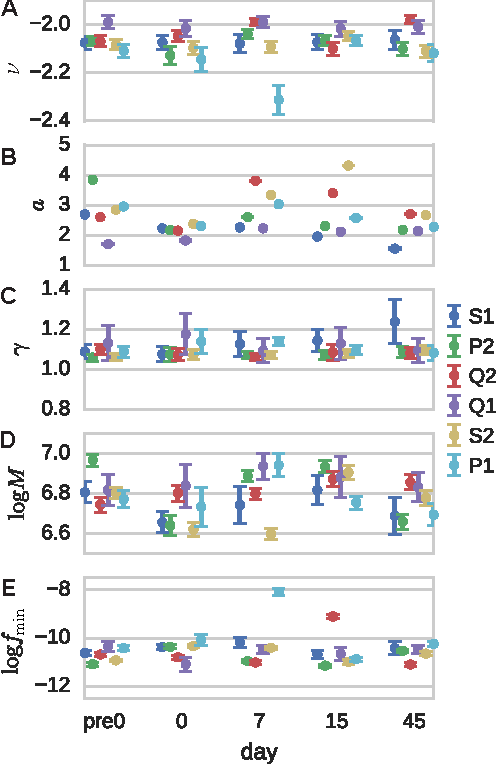
\includegraphics[width=.8\linewidth]{fig3_learnednullparas}
\centering{}
\caption{
  \emph{Inferred null model parameters}. Inferred values: for (A) the power-law exponent $\nu$ of the clone size distribution; (B) and (C) linear coefficient and exponent of the mean-variance relationship of the noise; (D) effective number of cells; and (E) minimal clonal frequency.
  Each point is inferred from a pair of replicates for a given donor and time point. Error bars are obtained by inverting the Hessian of the log-likelihood projected onto the hyperplane locally satisfying the normalization constraint.
\label{fig:nullparas_timeseries}}
\end{figure}


The inferred models can also be used to estimate the diversity of the entire repertoire (observed or unobserved).
The clone frequency distribution, $\rho(f)$, together with the estimate of $N$ can be used to estimate Hill diversities (see Methods):
\beq
D_\beta={\left(\sum_{i=1}^N f_i^\beta\right)}^{\frac{1}{1-\beta}}={\left(N\<f^\beta\>\right)}^{\frac{1}{1-\beta}}.
\eeq
In  \cref{fig:div_estimates}, we show the values, across donor and days, of three different diversities: species richness, i.e. the total number of clones $N$ ($\beta=0$); Shannon diversity, equal to the exponential of the Shannon entropy ($\beta=1$); and Simpson diversity, equal to the inverse probability that two cells belong to the same clone ($\beta=2$). In particular, estimates of $N\approx 10^9$ fall between the lower bound of $10^8$ unique TCRs reported in humans using extrapolation techniques \cite{Qi2014} and theoretical considerations giving upper-bound estimates of $10^{10}$ \cite{Lythe2016} or more \cite{Mora2019}.


\begin{figure}
%\includegraphics[width=\linewidth]{fig2_learnednullparas}
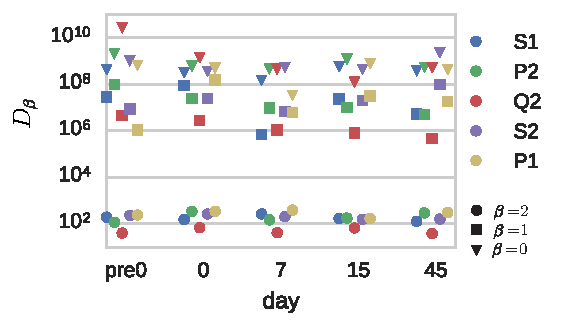
\includegraphics[width=\linewidth]{fig4_div_estimates}
\centering{}
\caption{\emph{Diversity estimates.} Shown are diversity estimates obtained from the Hill diversities, $D_\beta$, of the inferred clone frequency distributions for $\beta=0$ (estimated total number of clones, $N$), $\beta=1$ (Shannon entropy) and $\beta=2$ (Simpson index), across donors and days.
\label{fig:div_estimates}}
\end{figure}



\subsection*{Learning the repertoire dynamics from pairs of time points}

Now that the baseline for repertoire variation has been learned from replicates, we can learn something about its dynamics following immunization. The parameters of the expansion model (Eq.~\ref{eq:exp}) can be set based on prior knowledge about the typical fraction of responding clones and effect size. Alternatively, they can be inferred from the data using maximum likelihood estimation (Empirical Bayes approach). We define the likelihood of the read count pairs $(n,n')$ between time points $t$ and $t'$ as:
\beq
\begin{split}\label{eq:fullexp}
  &P_{\rm exp}(n,n'|\theta_{\rm null}, \theta_{\rm exp})=\\
  &\int_{f_{\rm min}}^1 \textrm{d}f\rho(f)\int \textrm{d}s\rho_{s}(s|\theta_{\rm exp})P(n|f, \theta_{\rm null})P(n'|fe^s, \theta_{\rm null}),
  \end{split}
  \eeq
where $\theta_{\rm exp}=\{\alpha,s_0,\bar s\}$ characterizes $\rho_s(s)$ (\cref{eq:exp}) with $\bar s$ parametrizing $\rho_{\textrm{exp}}(s)$, and where $\theta_{\rm null}=\hat \theta_{\rm null}$ is set to the value learned from replicates taken at the first time point $t$.
The maximum likelihood estimator is given by
\beq\label{eq:MLEexp}
\hat\theta_{\rm exp}=\argmax_{\theta_{\rm exp}} \prod_{i=1}^{N_{\rm obs}} \frac{P_{\rm exp}(n_i,n'_i|\hat\theta_{\rm null}, \theta_{\rm exp})}{1-P_{\rm exp}(0,0|\hat\theta_{\rm null}, \theta_{\rm exp})}.
\eeq
This maximization was performed via gradient-based methods. In Methods we give an example of a semi-analytic approach to finding the optimum using the expectation maximization algorithm. 

In addition to normalization at $t$, we also need to impose normalization at $t'$:
\beq
Z'=N	P(0,0)\langle f'\rangle_{\rho(f'|n+n^{\prime}=0)} + \sum_{i=1}^{N_{\textrm{obs}}}\langle f'\rangle_{\rho'(f'|n_i,n^{\prime}_i)},
\eeq
with $\rho(f'|n,n')\propto \int \textrm{d}f\rho(f)G(f'|f)P(n|f)P(n'|f')$ is the posterior distribution of the $f'$ given the read count pair. In practice, we impose $Z=Z'$, where $Z$ is the normalization of the first time point given by Eq.~\ref{eq:postnorm}.
Intuitively, this normalization constraint sets $s_0$ so that the expansion of a few clones is compensated by the slight contraction of all clones.

We first tested the method on synthetic data generated with the expansion model of Eq.~\ref{eq:fullexp}, with an exponentially distributed effect size for the expansion with scale parameter, $\bar{s}$:
\beq\label{eq:onesidedexp}
\rho_{\rm exp}(s')=\frac{1}{\bar s}e^{-s'/\bar s}\Theta(s'),
\eeq
where $\Theta(s')=1$ if $s'>0$ and $0$ otherwise (\cref{fig:diffexpr_ex1}A).
We simulated small, mouse-like and large, human-like repertoires (number of clones, $N=10^6$ and $N=10^9$; number of reads/sample $N_{\textrm{reads}}=10^4$ and $N_{\textrm{reads}}=2\cdot 10^6$, respectively), using $\nu=2$ and $f_{\textrm{min}}$ satisfying $N\langle f\rangle_{\rho(f)}$=1. For the parameter-free Poisson measurement model, we analyzed the differential expression model, \cref{eq:fullexp}, over a range of biologically plausible parameter values.  
In \cref{fig:diffexpr_ex1}B, we show the parameter space of the inference of a mouse repertoire generated with $(\bar{s}^*,\alpha^* )=(1.0,10^{-2})$ and $s_0=s_0(\alpha,\bar s)$ fixed by the normalization constraint $Z^\prime=Z$. The errors are distributed according to a diagonally elongated ellipse (or `ridge'), with a covariance following the inverse of the Hessian of the log-likelihood.
The imprecision of the parameter estimates is due to the small number of sampled responding clones. With
$\alpha^*=0.01$ and $N_{\rm obs}\approx 10^4$ sampled clones, only a few dozens responding clones are detected. For human-sized repertoires, millions of clones are sampled, which makes the inference much more precise (see \cref{fig:SM_reinf_diffexpr}).

Once learned, the model can be used to compute the posterior probability of a given expansion factor by marginalizing $f$, and using Bayes' rule, 
\begin{align}\label{eq:post}
	\rho(s|n,n^{\prime})\propto \rho_s(s)\int P(n|f)P(n^{\prime}|fe^s)\rho(f)\textrm{d}f.
\end{align}
We illustrate different posterior shapes from synthetic data as a function of the observed count pairs in \cref{fig:diffexpr_ex1}C. We see for instance that the width of the posterior narrows when counts are both large, and that  the model ascribes a fold-change of $s_0$ to clones with $n^{\prime} \lessapprox n$.

\begin{figure}
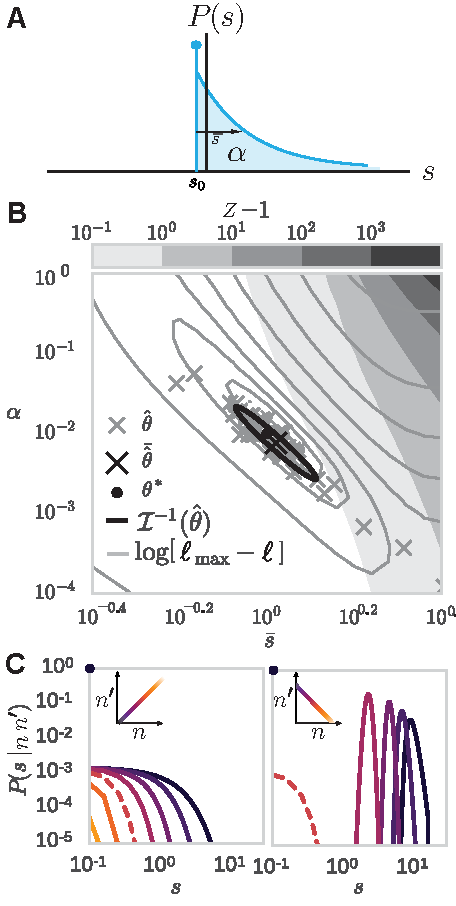
\includegraphics{fig5_diffexpr_eval}
\centering{}
\caption{
\emph{Inference of clonal expansion on synthetic data.}(A) The prior distribution of expansion log fold-changes, $\rho_s(s)$, is parametrized by a mean effect size, $\bar{s}$, describing the expansion of the responding fraction, $\alpha$ of the repertoire  (\cref{eq:onesidedexp}). 
Expansion is relative to a basal $s_0$ fixed by the normalization constraint.
(B) Re-inference of the expansion parameters from synthetic data generated with value $\theta_{\rm exp}^*=(\bar{s}^*,\alpha^* )=(1.0,10^{-2})$ (black dot). 
Maximums of the log-likelihood, $\hat\theta_{\rm exp}$, for 50 realizations (gray crosses), along with their average $\bar{\hat{\theta}}$ (black cross). 
The log-likelihood for one realization is shown over logarithmically-spaced gray contours decreasing from the maximum. 
The inverse Fisher information, $\mathcal{I}^{-1}$, for the same realization is shown as the black-lined ellipse centered at $\bar{\hat{\theta}}$, which provides a lower bound to the variance of our ML estimate. 
The gray scale contours increasing to the upper-right denote $Z^\prime/Z-1$, the excess in the used normalization. (C) Posteriors of the learned model, $\rho(s|n,n^{\prime})$ over pairs $(n,n^{\prime})$ for $n^{\prime}=n$, with $n$ varying over a logarithmically-spaced set of counts (left), and for $n^{\prime}$ given by the reverse order of this set (right). The black dot in both plots denotes the contribution of the non-responding component, $\propto \delta(s-s_0)$, to the posterior.
(Parameters: $N=10^6$, $\epsilon=10^{-2}$.)
\label{fig:diffexpr_ex1}
}
\end{figure}

Note that the value of the true responding fraction $\alpha$ is correctly learned from our procedure, regardless of our ability to tell with perfect certainty which particular clones responded. By contrast, a direct estimate of the responding fraction from the number of significantly responding clones, as determined by differential expression software such as EdgeR \cite{Robinson2010}, is likely to misestimate that fraction. We applied EdgeR to a synthetic repertoire of $N=10^9$ clones, a fraction $\alpha=0.01$ of which responded with mean effect $\bar s=1$, and sampled with $N_{\rm read}=10^6$. EdgeR found $6,880$ significantly responding clones (corrected p-value 0.05) out of $N_{\rm obs}=1,995,139 $, i.e. a responding fraction $6,880/1,995,139 \approx 3\cdot 10^{-3}$ of the observed repertoire, and a responding fraction $6,880/10^9\approx 7\cdot 10^{-6}$ of the total repertoire, underestimating the true fraction $\alpha=10^{-2}$.

\subsection*{Inference of the immune response following immunization} \label{sec:diffexpr}

Next, we ran the inference procedure on sequences obtained from human blood samples across time points following yellow fever vaccination. To guide the choice of prior for $s$, we plotted the histograms of the naive log fold-change $\ln n^{\prime}/n$ (\cref{fig:SM_snaive_hists}). These distributions show symmetric exponential tails, motivating us to model the statistics of expansion factors as:
\beq\label{eq:symmexp}
\rho_{\rm exp}(s)=\frac{1}{2\bar s}e^{-|s|/\bar s},
\eeq
with typical effect size $\bar{s}$.

We applied the inference procedure (Eq.~\ref{eq:MLEexp}) between the repertoires taken the day of vaccination (day 0), and at one of the other time points (day -7, day 7, day 15, and day 45) after vaccination. Since there are two replicates at each time point, we can make 4 comparisons between any pair of time points.

Same-day comparisons (day 0 vs day 0) gave effectively zero mean effect sizes ($\bar s<0.1$, below the discretization step of the integration procedure), as expected (Fig.~\ref{fig:diffexpr_ex2}). Comparisons with other days yielded inferred values of $\alpha$ and $\bar s$ distributed along the same  `ridge' (Fig.~\ref{fig:diffexpr_ex2}), as observed on synthetic data (\cref{fig:diffexpr_ex1}). The mean effect size $\bar s$ is highest at day 15, where the peak of the response occurs, but is also substantially different from 0 at all time points except day 0 (including before vaccination at day $-7$), with often high values of $\alpha$. We speculate that these fluctuations reflect natural variations of the repertoire across time, as well as experimental batch effects. As a consequence of the natural diversity, 
values of the responding fraction $\alpha$ are not learned with great precision, as can be seen from the variability across the 4 choices of replicate pair, and are probably gross overestimations of the true probability that a naive T cell responds to an infection, which is believed to be of order $10^{-5}-10^{-3}$ \cite{Boer1993}.


\begin{figure}
\includegraphics[width=\linewidth]{sbar_alp_vals_linscale}
\centering{}
\caption{
\emph{Application to yellow fever vaccination data.} Optimal values of $\alpha$ and $\bar{s}$ across all 6 donors and days relative to the day of vaccination (day 0). Inset shows the same data on a logarithmic scale for comparison with \cref{fig:diffexpr_ex1}b. Comparisons with days other than 0 fall on straight line (dashed line).
\label{fig:diffexpr_ex2}
}
\end{figure}


\subsection*{Identifying responding clones}

The posterior probability on expansion factors $\rho(s|n,n')$ (Eq.~\ref{eq:post}) can be used to
study the fate and dynamics of particular clones. For instance, we can
identify responding clones as having a low posterior probability of being not expanding $P_{\rm null}=\rho(s\leq 0|n,n')<0.025$. $P_{\rm null}$ is the Bayesian counterpart of a p-value but differs from it in a fundamental way: it gives the probability that expansion happened given the observations, when a p-value would give the probability of the observations in absence of expansion.  We can define a similar criterion for contracting clones.

To get the expansion or contraction factor of each clone, we can compute the posterior average and median, $\<s\>_{n,n'}=\int \textrm{d}s\,s \rho(s|n,n')$ and $s_{\rm median}$ ($F(s_{\rm median}|n,n')=0.5$, for the cumulative density function, $F(s|n,n')=\int_{-\infty}^s\rho(\tilde{s}|n,n')\textrm{d}\tilde{s}$),  corresponding to our best estimate for the log fold-change.
In \cref{fig:SM_smed_snaive}, we show how the median Bayesian estimator differs from the naive estimator $s_{\textrm{naive}}=\ln n^{\prime}/n$. While the two agree for large clones for which relative noise is smaller, the naive estimator over-estimates the magnitude of log fold-changes for small clones because of the noise. The Bayesian estimator accounts for that noise and gives a more conservative and more realistic estimate.

\begin{figure*}
\includegraphics[width=\textwidth]{fig8_volc_plus}
\centering{}
\caption{
\emph{Identifying responding clones}. (A) Plot of confidence of expanded response versus average effect size. A significance threshold is placed according to $P_{\textrm{null}}=0.025$, where $P_{\textrm{null}}=P(s\leq 0)$. (B) The same threshold for significant expansion in $(n,n^\prime)$-space with identified clones highlighted in red. (C) The optimal values of $\alpha$ and $\bar{s}$ for donor S2 and day-0 day-15 comparison for 3 replicates (square markers). The background heat map is the list overlap (the size of the intersection of the two lists divided by the size of their union) between a reference list obtained at the optimal $\hat\theta_{\rm exp}$ (black dot) and lists obtained at non-optimal $\theta_{\rm exp}$. (D) Mean posterior log fold-change $\<s\>_{\rho(s|n,n')}$ as a function of precursor frequency.
\label{fig:volcano}}
\end{figure*}

In \cref{fig:volcano}A, we show a `volcano' plot showing how both $P_{\rm null}$ and $\<s\>_{n,n'}$ vary as one scans values of the count pairs $(n,n')$. \Cref{fig:volcano}B shows the all count pairs $(n,n')$ between day $0$ and day $15$ following yellow fever vaccination, with red clones above the significance threshold line $P_{\rm null}=0.025$ being identified as responding.

Given the uncertainty in the expansion model parameters $\theta_{\rm exp}=(\bar s,\alpha)$, we wondered how robust our list of responding clonotypes was to those variations. In \cref{fig:volcano}C, we show the overlap of lists of strictly expanding clones ($P(s\leq 0|n,n')<0.025$) as a function of $\theta_{\rm exp}$, relative to the optimal value $\hat\theta_{\rm exp}$ (black circle). The ridge of high overlap values exactly mirrors the ridge of high likelihood values onto which the learned parameters fall (\cref{fig:diffexpr_ex2}). Values of $\hat \theta_{\rm exp}$ obtained for other replicate pairs (square symbols) fall onto the same ridge, meaning that these parameters lead to virtually identical lists of candidates for response.

The list of identified responding clones can be used to test hypotheses about the structure of the response. For example, recent work has highlighted a power law relationship between the initial clone size and clones subsequent fold change response in a particular experimental setting \cite{Mayer2019}. We can plot the relationship in our data as the posterior mean log fold change versus the posterior initial frequency, $f$ (\cref{fig:volcano}D). While the relationship is very noisy, emphasizing the diversity of the response, it is consistent with a decreasing dependency of the fold change with the clone size prior to the immune response.

The robustness of our candidate lists rests on their insensitivity to the details of how the model explains typical expansion. In \cref{fig:posteriors}, we show how the posterior belief varies significantly for count pairs $(0,n^\prime)$, $n^\prime>0$, across a range of values of $\bar{s}$ and $\alpha$ passing along the ridge of plausible models (\cref{fig:volcano}C). A transition from a low to high value of the most probable estimate for $s$ characterizes their shapes and arises as $\bar{s}$ becomes large enough that expansion from frequencies near $f_\textrm{min}$ is plausible, and the dominant mass of clones there makes this the dominate posterior belief. Thus, these posteriors are shaped by $\rho_s(s)$ at low $\bar{s}$, and $\rho(f)$ at high $\bar{s}$. Our lists vary negligibly over this transition, and thus are robust to it.



\section*{Discussion}

Our probabilistic framework describes two sources of variability in clonotype abundance from repertoire sequencing experiments: biological repertoire variations and spurious variations due to noise. We found that in a typical experiment, noise is over-dispersed relative to Poisson sampling noise. This makes the use of classical difference tests such as Fisher's exact test or a chi-squared test inappropriate in this context, and justifies the development of specific methods.

As a byproduct, our method learned the properties of the clone size distribution, which is consistent with a power law of exponent $\approx -2.1$ robust across individuals and timepoints, consistent with previous reports \cite{Mora2016e,Gerritsen_thesis,Greef2019}. Using these parameters, various diversity measures could be computed, such as the species richness ($10^8$--$10^9$), which agrees with previous bounds \cite{Qi2014,Lythe2016}, or the ``true diversity'' (the exponential of the Shannon entropy), found to range between $10^6$ and $10^8$.

The proposed probabilistic model of clonal expansion is described by two parameters: the fraction of clones that respond to the immune challenge, and the typical effect size (log fold-change). While these two parameters were difficult to infer precisely individually, a combination of them could be robustly learned. Despite this ambiguity in the model inference, the list of candidate responding clonotypes is largely insensitive to the parameter details. For clonotypes that rose from very small read counts to large ones, the inferred fold-change expansion factor depended strongly on the priors, and resulted from a delicate balance between the tail of small clones in the clone size distribution and the tail of large expansion events in the distribution of fold-changes.

While similar approaches have been proposed for differential expression analysis of RNA sequencing data \cite{Robinson2008,Robinson2010,Anders2010,Love2014}, the presented  framework was specifically built to address the specific challenges of repertoire sequencing data. Here, the aim is to count proliferating cells, as opposed to evaluating average expression of genes in a population of cells. We specifically describe two steps that translate cell numbers into the observed TCR read counts: random sampling of cells that themselves carry a random number of mRNA molecules, which are also amplified and sampled stochastically. Another difference with previous methods is the explicit Bayesian treatment, which allows us to calculate a posterior probability of expansion, rather than a less interpretable p-value.

Here we applied the presented methodology to an acute infection. We have previously shown that it can successfully identify both expanding (from day 0 to 15 after vaccination) and contracting (from day 15 to day 45) clonotypes after administering a yellow fever vaccine. However the procedure is more general and can also be extended to be used in other contexts. For instance, this type of approach could be used to identify response in B-cells during acute infections, by tracking variations in the size of immunoglobulin sequence lineages (instead of clonotypes), using lineage reconstruction methods such as Partis~\cite{Ralph2016a}.
The framework could also be adapted to describe not just expansion, but also switching between different cellular phenoypes during the immune response, {\em e.g.} between the naive, memory, effector memory, {\em etc.} phenotypes, which can obtained by flow-sorting cells before sequencing \cite{Minervina2019}. Another possible application would be to track the clones across different tissues and organs, and detect migrations and local expansions \cite{Kadoki2017}.

The proposed framework is not limited to identifying a response during an acute infection, but can also be used as method for learning the dynamics from time dependent data even in the absence of an external stimulus~\cite{Chu2019}. Here we specifically assumed expansion dynamics with strong selection. However, the propagator function can be replaced by a non-biased random walk term, such as genetic drift. In this context the goal is not to identify responding clonotypes but it can be used to discriminate different dynamical models in a way that accounts for different sources of noise inherently present in the experiment. Alternatively, the framework can also be adapted to describe chronic infections such as HIV \cite{Nourmohammad2019}, where expansion events may be less dramatic and more continuous or sparse, as the immune system tries to control the infection over long periods of time.


%\begin{itemize}
%	\item  Summary:
%		\begin{itemize}
%			\item  used replicates to fix noise model: good fits for over-dispersed models; fairly universal across days/donors
%			\item  inferred repertoire change distributions: variable on ridge over replicates; consistent across days
%			\item  used to determine significantly expanded clones: threshold in prob expansion leads to threshold in (n,n')-space; list robust to replicate variability and details of priors and their interaction.
%		\end{itemize}
%	\item  Natural variation results and discussion:
%		\begin{itemize}
%			\item  Implications of universal parameters
%			\item  frequency power law tightly constrained by data. Implications...
%		\end{itemize}
%	\item  diffexpr results and discussion:
%		\begin{itemize}
%			\item  data strongly constrains prior expansion, not contraction or responding fraction. Implications...
%			\item  the relevance of homeostatis (normalization).
%			\item  Power and weakness of Bayes approach: robustness of list to details; inability to precisely pin down parameters (e.g. alpha)
%
%		\end{itemize}
%    \item  application results and discussion:
%		\begin{itemize}
%			\item  posterior sensitivity to balance between $\nu$ (prior for maximum expansion) and $\bar{s}$ (prior for characteristic expansion) in $(0,n)$ and $(n,0)$ pairs.
%			\item  sensitivity of resulting tables. Note validation in Misha's paper.
%		\end{itemize}
%	\item  Clinical use (reference Misha paper)
%	\item  drawbacks of approach: need replicate data, ...
%\end{itemize}





\section*{Methods}


%\appendix

\subsection*{Code}
All code used to produce the results in this work was custom written in Python 3 and is publicly available online at \url{https://github.com/mptouzel/bayes_diffexpr}.

%\subsection*{Clone frequency model}
%Based on previous observations \cite{Weinstein2009,Mora2010,Mora2016e}, $\rho(f)$ is set as a power-law, i.e. $\rho(f)\propto f^{-\nu}$. The bounded domain $f_{\textrm{min}}\leq f \leq 1$ makes the proportionality factor dependent on $f_{\textrm{min}}$ and $\nu$.

%\subsection*{Noise model}
%We considered three different statistical models of cells and mRNA molecules contained in a sample. These used a negative binomial distribution, with parametrized over-dispersion: $\mathrm{NegBin}(\mu, \sigma^2=\mu+a \mu^{\gamma})$ with $a>0$ the coefficient and $\gamma>1$ the power controlling the over-dispersion, and a Poisson distribution, $\mathrm{Poisson}(\lambda)$ with scale parameter $\lambda$.
 
%The highest scoring model is of cells sampled from a negative binomial, followed mRNA molecules sampled from a Poisson distribution. A clone of size $f$ appears in a sample containing $M$ lymphocytes on average as $\mu=fM$ cells. 
%To account for over-dispersed count statistics, the number of cells is set to be Negative-Binomial distributed with mean $fM$ and variance $fM+a (fM)^{\gamma}$, with $a>0$ the coefficient and $\gamma>1$ the power controlling the over-dispersion. 
%For each clone, the number $n$ of detected mRNA molecules (i.e. UMI) is distributed according to a Poisson distribution with mean $\lambda=mN_{\textrm{reads}}/M$, where $N_{\textrm{reads}}/M$ is the average number of UMI per cell, obtained using the observed total number of molecules, $N_{\textrm{reads}}$ and $m$ is the unobserved number of cells of that clone in the sample.
  
%We inferred the parameters of this noise model, $\theta_\textrm{null}=\{f_\textrm{min},\nu,a,\gamma,M\}$, from day-0 replicates by maximizing the likelihood of the observed count pairs, $(n,n^{\prime})$, subject to the normalization constraint \ref{eq:postnorm}. The likelihood, $P(n,n^{\prime}|\theta_{\textrm{null}})$, is obtained by marginalizing over $m,m'$, and $f$.
%We implemented this constrained maximization using the scipy package implementation of the sequential least squares programming method in python.  
%$n\sim \mathrm{Poisson}(m N/M)$, $m\sim \mathrm{NegBin}(fM,fM+a (fM)^{\gamma})$, for each replicate, and $f\sim\rho$ is common to both replicates. F

\subsection*{Normalization of the clonal frequencies}\label{sec:normal}
Here we derive the condition for which the normalization in the joint density is implicitly satisfied. The normalization constant of the joint density is
\begin{equation}
	\mathcal{Z}=\int_{f_\textrm{min}}^1\cdots\int_{f_\textrm{min}}^1\prod_{i=1}^N \rho(f_i)\delta(Z-1)\textrm{d}^N\vec{f} \;\label{eq:joint},
\end{equation}
with $\delta(Z-1)$ being the only factor preventing factorization and explicit normalization. Writing the delta function in its Fourier representation factorizes the single constraint on $\vec{f}$ into $N$ Lagrange multipliers, one for each $f_i$,
\begin{align}
	\delta(Z-1)&=\int_{-i\infty}^{i\infty} \frac{\textrm{d} \mu}{2 \pi}e^{\mu(Z-1)}  \\
	&=\int_{-i\infty}^{i\infty} \frac{\textrm{d} \mu}{2 \pi}e^{-\mu}\prod_{i=1}^N e^{\mu f_i} \;.
\end{align}
Crucially, the multi-clone integral in \cref{eq:joint} over $\vec{f}$ then factorizes. Exchanging the order of the integrations we obtain
\begin{equation}
	\mathcal{Z}=\int_{-i\infty}^{i\infty} \frac{\textrm{d} \mu}{2 \pi} e^{-\mu} \langle e^{\mu f}\rangle^N\;,\label{eq:bigZ}
\end{equation}
with $\langle e^{\mu f}\rangle=\int_{f_\textrm{min}}^1\rho(f)e^{\mu f}\textrm{d}f$. Now define the large deviation function, $I(\mu):=-\frac{\mu}{N}+\log \langle e^{\mu f}\rangle$, so that 
\begin{equation}
	\mathcal{Z}=\int_{-i\infty}^{i\infty} \frac{\textrm{d} \mu}{2 \pi} e^{-N I(\mu)}\;.\label{eq:largedev}
\end{equation}
Note that $I(0)=0$. With $N$ large, this integral is well-approximated by the integrand's value at its saddle point, located at $\mu^*$ satisfying $I'(\mu^*)=0$.  Evaluating the latter gives
\begin{align}
	\frac{1}{N}&=\frac{\langle f e^{\mu^* f}\rangle}{\langle e^{\mu^* f}\rangle}\;.
\end{align} 
If the left-hand side is equal to $\langle f\rangle$, the equality holds only for $\mu^*=0$ since expectations of products of correlated random variables are not generally products of their expectations. 
In this case, we see from \cref{eq:largedev} that $\mathcal{Z}=1$, and so the constraint $N\langle f\rangle=1$ imposes normalization.
% \begin{align}
% 	\langle g(\vec{f})\rangle_{\rho_N(\vec{f})}&=\int_{f_\textrm{min}}^1\cdots\int_{f_\textrm{min}}^1\prod_{i=1}^N \rho(f)\frac{1}{2 \pi} \int_{-i\infty}^{i\infty} e^{i \mu(Z-1)} \textrm{d} \mu \textrm{d}^N\vec{f} g(\vec{f})\\
% 	\int_{f_\textrm{min}}^1\cdots\int_{f_\textrm{min}}^1\prod_{i=1}^N \rho(f)\frac{1}{2 \pi} \int_{-i\infty}^{i\infty} e^{i \mu(Z-1)} \textrm{d} \mu \textrm{d}^N\vec{f} g(\vec{f})\;.
% \end{align}

\subsection*{Null model sampling}\label{sec:null_sampling}
The procedure for null model sampling is summarized as (1) fix main model parameters, (2) solve for remaining parameters using the normalization constraint, $N \langle f \rangle=1$, and (3) starting with frequencies, sample and use to specify the distribution of the next random variable in the chain.

In detail, we first fix: (a)
%\begin{itemize}
%\item
the model parameters $\{\alpha,M,a,\gamma\}$, excluding $f_{\textrm{min}}$;
% Separate $M$, $a$, and $\gamma$ values could be defined for the reference and test condition, respectively. The empirical $P(n,n^{\prime})$ for replicate data was found to be highly symmetric in $n$ and $n^{\prime}$ across donors, however, supporting the assumption of a single acquisition model and so we neglect this complication. 
% \item
(b) the desired size of the full repertoire, $N$;
%Together with the model prediction of capture efficiency, $1-P(0,0)$, this gives the number of clones we should sample, $N_{\textrm{\textrm{obs}}}$, via $N_{\textrm{\textrm{obs}}}=N(1-P(0,0))$, 
% \item
(c) the sequencing efficiency (total sample reads/total sample cells), $\epsilon$. From this we get the effective total sample reads, $N^{\textrm{eff}}_{\textrm{reads}}=\epsilon M$, which converts a clone's frequency to the average number of cells it appears with in the sample.
% (We could in fact define two sequencing efficiencies, one for each replicate, leading to different effective total number of reads in each replicate).
Note that the actual sampled number of reads is stochastic and so will differ from this fixed value.
%\end{itemize}

We then solve for remaining parameters. Specifically, $f_{\textrm{min}}$ is fixed by the constraint that the average sum of all frequencies, under the assumption that their distribution factorizes, is unity:
\begin{equation}
% 	P(0,0)N\langle f\rangle_{\rho(f|n+n^{\prime}=0)} + N_{\textrm{\textrm{obs}}} \langle f\rangle_{\rho(f|n+n^{\prime}>0)} = 1
	N \langle f\rangle_{\rho(f)}=1
\end{equation}
This completes the parameter specification.

We then sample from the corresponding chain of random variables.
Sampling the chain of random variables of the null model can be performed efficiently by only sampling the $N_{\textrm{obs}}=N(1-P(0,0))$ observed clones. This is done separately for each replicate, once conditioned on whether or not the other count is zero. 
Samples with 0 molecule counts can in principle be produced with any number of cells, so cell counts must be marginalized when implementing this constraint. We thus used the conditional probability distributions $P(n|f)=\sum_{m}P(n|m)P(m|f)$ with $m,n=0,1,\dots$. $P(n^\prime|f)$ is defined similarly. Note that these two conditional distributions differ only in their average number of UMI per cell, $N_{\textrm{read}}/M$, due to their differing number of observed total number of molecules, $N_{\textrm{read}}$. Together with $\rho(f)$, these distributions form the full joint distribution, which is conditioned on the clone appearing in the sample, i.e. $n+n^{\prime}>0$ (denoted $\mathcal{O}$), 
\begin{align}
	P(n,n^{\prime},f|\mathcal{O})= \frac{P(n|f)P(n^{\prime}|f)\rho(f)}{1-\int{\textrm{d}f \rho(f)\textrm{d}f P(n=0|f)P(n^{\prime}=0|f)}}\;,  
\end{align}
with the renormalization accounting for the fact that $(n,n^{\prime})=(0,0)$ is excluded. The 3 quadrants having a finite count for at least one replicate are denoted $q_{x0}$, $q_{0x}$, and $q_{xx}$, respectively. Their respective weights are
\begin{align}
	P(q_{x0}|\mathcal{O})&=&\sum_{n>0}\int{\textrm{d}f P(n,n^{\prime}=0,f|\mathcal{O})}\;,\\
	P(q_{0x}|\mathcal{O})&=&\sum_{n^{\prime}>0}\int{\textrm{d}f P(n=0,n^{\prime},f|\mathcal{O})}\;,\\
	P(q_{xx}|\mathcal{O})&=&\sum_{\substack{n>0,\\n^{\prime}>0}}\int{\textrm{d}f P(n,n^{\prime},f|\mathcal{O})}.
\end{align}
Conditioning on $\mathcal{O}$ ensures normalization, $P(q_{x0}|\mathcal{O})+P(q_{0x}|\mathcal{O})+P(q_{xx}|\mathcal{O})=1$. Each sampled clone falls in one the three regions according to these probabilities. Their clone frequencies are then drawn conditioned on the respective region, 
\begin{align}
	P(f|q_{x0})&=&\sum_{n>0}P(n,n^{\prime}=0,f|\mathcal{O})/P(q_{x0}|\mathcal{O})\;,\\
	P(f|q_{0x})&=&\sum_{n^{\prime}>0}P(n=0,n^{\prime},f|\mathcal{O})/P(q_{0x}|\mathcal{O})\;,\\
	P(f|q_{xx})&=&\sum_{{n>0,n^{\prime}>0}}P(n,n^{\prime},f|\mathcal{O})/P(q_{xx}|\mathcal{O}).
\end{align}

Using the sampled frequency, a pair of molecule counts for the three quadrants are then sampled as $(n,0)$, $(0,n^{\prime})$, and $(n,n^{\prime})$, respectively, with $n$ and $n^{\prime}$ drawn from the renormalized, finite-count domain of the conditional distributions, $P(n|f,n>0)$. 

% Using the sampled frequency, a pair of number of cells $(m,m^{\prime})$ is obtained. For $q_{x0}$, $m$ is sampled from $P(m|f,n>0)$ and $m^{\prime}$ sampled from $P(m^{\prime}|f,n^{\prime}=0)$ with 
% \begin{align}
% 	P(m|f,n>0)&=&\frac{\sum_{n>0}P(m,n|f)}{\sum_{\substack{n>0,\\m}}P(m,n|f)}\;,\\
% 	P(m^{\prime}|f,n^{\prime}=0)&=&\frac{P(m^{\prime},n^{\prime}=0|f)}{\sum_{m^{\prime}}P(m^{\prime},n^{\prime}=0|f)}\;,
% \end{align}
% with $P(m_i,n_i|f)=P(n_i|m_i)P(m_i|f)$, for $i=1,2$. Note that by construction here, $m>0$, since $P(n>0|m=0)=0$.
% The procedure is similar for frequencies sampled in $q_{0x}$. For frequencies sampled in $q_{xx}$, cell count pairs $(m,m^{\prime})$ are sampled from $P(m|f,n>0)$ and $P(m^{\prime}|f,n^{\prime}>0)$, respectively. 
% 
% Molecule counts for the three quadrants are then sampled as $(n,0)$, $(0,n^{\prime})$, and $(n,n^{\prime})$, respectively, with $n$ and $n^{\prime}$ drawn from the renormalized, finite-count domain of the conditional distributions, $P(n|m)$ and $P(n^{\prime}|m^{\prime})$, respectively, with $m>0$ and $m^{\prime}>0$. 

Using this sampling procedure we demonstrate the validity of the null model and its inference by sampling across the observed range of parameters and reinferring their values (see \cref{fig:SM_reinfer_null}).


\subsection*{Differential model sampling}\label{sec:diffexpr_sampling}
Since the differential expression model involves expansion and contraction in the test condition, some normalization in this condition is needed such that it produces roughly the same total number of cells as those in the reference condition, consistent with the observed data. One approach (the one taken below) is to normalize at the level of clone frequencies. 
Here, we instead perform the inefficient but more straightforward procedure of sampling all $N$ clones and discarding those clones for which $(n,n^{\prime})=(0,0)$. A slight difference in the two procedures is that $N_{\textrm{obs}}$ is fixed in the former, while is stochastic in the latter.


%\subsection*{Direct sampling}
The frequencies of the first condition, $f_i$, are sampled from $\rho(f)$ until they sum to 1 (i.e. until before they surpass 1, with a final frequency added that takes the sum exactly to 1). An equal number of log-frequency fold-changes, $s_i$, are sampled from $\rho(s)$. The normalized frequencies of the second condition are then $f'_i=f_ie^{s_i}/\sum_j f_je^{s_j}$.  Counts from the two conditions are then sampled from $P(n|f)$ and $P(n^{\prime}|f')$, respectively. Unobserved clones, i.e. those with $(n,n^{\prime})=(0,0)$, are then discarded.

% \subsubsection*{Effective sampling}
% For an efficient implementation, the procedure should avoid sampling the numerous clones that produce $(n,n^{\prime})=(0,0)$, since these are discarded. Such a procedure follows. 
% 
% First, the $(f,s)$-plane is partitioned into two regions, $D=\{(f,s)|f<f_0,fe^s<f_0\}$ and its complement, $\bar D$, with $f_0$ chosen such that clones sampled from $\bar D$ are often \textit{observed}, i.e. $n+n^{\prime}>0$ (a minority of clones sampled in $\bar D$ will nevertheless give $n+n^{\prime}=0$; these are discarded). In contrast, frequencies sampled from $D$ will be small, so that most will be unobserved, and we must condition on the clone being observed when sampling from this regime. Moreover, their average is unaffected by the long-tailed behaviour of the distribution in the large-frequency regime and thus is well-approximated by the corresponding ensemble average. We use this latter fact when computing the renormalization of the frequencies of the second condition. 
% 
% We compute the mass in $D$ as $P_D=\int_f \textrm{d}f\rho(f)\sum_s \rho(s) \mathbb{1}((f,s)\in D)$.
% 
% We sample $(f,s)$ in $\bar D$ until the sum of the first condition^{\prime}s frequencies, $\sum_i f_i$ added to the expected sum in $D$, $P_D N_{cl}\langle f\rangle_{P(f|D)}$, equals 1,
% \begin{align}
% 	1=\sum_{i=1}^{N_{\bar D}} f_i + P_D N_{cl}\langle f\rangle_{P(f|D)}\;,
% \end{align}
% where $N_{cl}$ is the total number of clones in the repertoire. The number sampled from $\bar D$, $N_{\bar D}$, is determined from that expression self-consistently by substituting $N_{cl}=N_{\bar D}/(1-P_D)$ obtained from $N_{\bar D}+P_D N_{cl}\equiv N_{cl}$. The normalization for the second condition^{\prime}s frequencies is then 
% \begin{align}
% 	Z=\sum_{i=1}^{N_{\bar D}} f_ie^{s_i} + P_D N_{cl}\langle fe^s\rangle_{P(f,s|D)}
% \end{align}
% such that the second condition^{\prime}s frequencies are ${f_i'=f_ie^{s_i}/Z}$. Molecule counts are then sampled from $P(n|f)$ and $P(n^{\prime}|f')$.  
% 
% We then sample from $D$ conditioned on the clone being observed, i.e. having produced a finite number of molecules in either of the two conditions. We thus sample $N_D=P(n+n^{\prime}>0|D)P_D N_{cl}$ clones from $P(f,s|D,n+n^{\prime}>0)$. To avoid having to sample over the joint distribution of $n$ and $n^{\prime}$, we condition on the 3 regions of finite counts in both conditions, $(n,0)$, $(0,n^{\prime})$, and $(n,n^{\prime})$, in which $n$ and $n^{\prime}$ can be sampled independently. 
% Note the presence of the normalization factor, $Z$, in 
% \begin{align}
% 	P(n+n^{\prime}>0|D)=\int_f \textrm{d}f\rho(f)\sum_s \rho(s)(1-P(n=0|f)P(n^{\prime}=0|f'=fe^s/Z))\;.
% \end{align}
% and
% \begin{align}
% 	P(f,s|D,n+n^{\prime}>0)=\frac{\rho(f)\rho(s)(1-P(n=0|f)P(n^{\prime}=0|f'=fe^s/Z))}{P(n+n^{\prime}>0|D)P_D}\;.
% \end{align}
% We then concatenate the $N_D$ sampled counts from $D$ and the $N_{\bar D}$ sampled counts (with $(n,n^{\prime})=(0,0)$ realizations discarded) from $\bar D$ to obtain the full data set.  

% \subsection*{Null Model Inference}
% Given a data set, $\mathcal{D}=\{(n_i,n^{\prime}_i)\}_{i=1}^{N_{\textrm{obs}}}$, we infer the parameters of the null model, $\Theta_{\textrm{null}}=(\alpha,a,\gamma,M,f_{\textrm{min}})$ by maximizing the marginal likelihood of the observable model, $P(n,n^{\prime}|n+n^{\prime}>0,\Theta_{\textrm{null}})$, subject to the normalization constraint$, N\langle f\rangle_{\rho(f)}=1$, where $N=N_{\textrm{obs}}/(1-P(0,0))$. Since in this case we have access to a realization, we could instead normalize conditioned on this realization. Since, 
% \begin{equation*}
% 	N\sum_{(n,n^{\prime})>0}P(n,n^{\prime})\approx N\sum_{(n,n^{\prime})\in \mathcal{D}}\frac{\#(n,n^{\prime})}{N}\equiv \sum_{i}^{N_{\textrm{obs}}}
% \end{equation*}
% we then have
% \begin{equation}
% 	1=N\langle f\rangle_{\rho(f|\mathcal{D})}
% 							   = P(0,0)N\langle f\rangle_{\rho(f|n+n^{\prime}=0)} + \sum_{i}^{N_{\textrm{obs}}}\langle f\rangle_{\rho(f|n_i,n^{\prime}_i)}\;.
% \end{equation}

% \subsection*{Differential expression model definition}
% We introduce a selection factor $s$ defined as the log-frequency fold-change between a clone's frequency on one day, $f$, and that on another, $fe^s$, and define $P(n,n^{\prime}|s,\theta_n)$ as before, but replacing $f$ by $fe^s$ in the definition of $m^{\prime}$. Given a prior distribution  $P(s|\theta_s)$ over $s$ parametrized by a set of parameters $\theta_s$ distinct from $\theta_n$, we used Bayes rule to obtain the posterior log-frequency fold-change probability function given an observed count pair, $P(s|n,n^{\prime},\theta_n,\theta_s)$. We set the values of the parameters $\theta_s$ of this prior by again maximizing the likelihood of the count pair data given the model over $\theta_s$, $\int P(n,n^{\prime}|s,\theta_n)P(s|\theta_s)\textrm{d}s$.
% 
% We explored a family of priors expressible as 
% \begin{eqnarray}
% 	P(s|\theta_s)&=&\frac{\alpha \beta}{Z_+}e^{-\frac{|s-s_0|}{s_+}}\Theta(s-s_0) \nonumber\\
% 	&&+\frac{\alpha (1-\beta)}{Z_-}e^{-\frac{|s-s_0|}{s_-}}\Theta(s_0-s) \\
% 	&&+(1-\alpha)\delta(s-s_0)\;, \label{eq:genPs}\nonumber
% \end{eqnarray}
% with $Z_{\pm} \sim s_{\pm}$ (see  \cref{fig:Ps}) so that in the most general prior, $\theta_s=(s_-,s_+,\alpha,\beta,s_0)$. See table \ref{Tbl1:Priors} for reduced-parameter versions of this model that we considered.


\subsection*{Obtaining diversity estimates from the clone frequency density}\label{sec:infer_div}
For a set of clone frequencies, $\{f_i\}_{i=1}^{N}$, the Hill family of diversities are obtained from the R\'enyi entropies, as $D_\beta=\exp H_\beta$, with $H_\beta=\frac{1}{1-\beta}\ln \left[ \sum_{i=1}^N f_i^{\beta}\right]$. We use $\rho(f)$ to compute their ensemble averages over $f$, again under the assumption that the joint distribution of frequencies factorizes. We obtain an estimate for $D_0=N$ using the model-derived expression, $N_{\textrm{obs}}+P(n=0)N=N$, where $N_{\textrm{obs}}$ is the number of clones observed in one sample, and $P(n=0)=\int_{f_{\textrm{min}}}^1 P(n=0|f)\rho(f)\textrm{d}f$. For $\beta=1$, we compute $\exp (N\langle -f\log f \rangle_{\rho(f)})$ and for $\beta=2$, we use $1/\left(N\langle f^2\rangle_{\rho(f)}\right)$.


% \begin{align}
% 	P(f,s|n,n^{\prime})&=&\frac{P(n,n^{\prime},f,s)}{\int\textrm{d}f\int\textrm{d}s P(n,n^{\prime},f,s)}
% \end{align}
% and using this, $P(f|n+n^{\prime}>0)=\int\textrm{d}s P(f,s|n,n^{\prime})$. 
% 
% \re{need to mention that the realization specific constraints are used here.}
% 
% The shift enters in $P(n,n^{\prime},f,s)=P(n|f)P(n^{\prime}|f,s)\rho(f)\rho_{s_0}(s)$ via $\rho_{s_0}(s)$. A convenient change of variables $s\leftarrow\Delta s+s_0$ maps $\rho_{s_0}(s)$ to $\rho_{0}(\Delta s)$, upon which
% \begin{align}
% 	\langle fe^s \rangle &=&\int{ \textrm{d}f \sum_{\Delta s} fe^{\Delta s+s_0} P(n|f)P(n^{\prime}|f,\Delta s+s_0)\rho(f)\rho_{0}(\Delta s)} \\
% 						 &=&e^{s_0}\int{ \textrm{d}f \sum_{\Delta s} fe^{\Delta s} P(n|f)P(n^{\prime}|f,\Delta s+s_0)\rho(f)\rho_{0}(\Delta s)}\;.
% \end{align}
% Denoting the remaining integral, $\tilde{\langle fe^s \rangle}$, and performing the same change of variables on $\langle f \rangle$,
% \begin{align}
% 	\langle f \rangle &=&\int{ \textrm{d}f \sum_{\Delta s} f             P(n|f)P(n^{\prime}|f,\Delta s+s_0)\rho(f)\rho_{0}(\Delta s)}\;,
% \end{align}
% the condition can be written as $s_0=\ln \tilde{\langle fe^s \rangle} - \ln \langle f \rangle$. To obtain $s_0$ from this implicit equation, we apply an iterative scheme beginning with $s_0=0$. We compute $P(n^{\prime}|f,\Delta s+s_0)$, and then the latter expression supplies $s_0$ in the next iteration. In practice, we take a bounded range of $\Delta s$ symmetric around 0. Thus, the only factor containing shift information is $P(n^{\prime}|f,\Delta s+s_0)$ appearing in both $\tilde{\langle fe^s \rangle}$ and $\langle f \rangle$. However, for self-consistent numerics, the $e^{\Delta s}$ factor must be defined over a shifted domain.

\subsection*{Inferring the differential expression prior}\label{sec:EM}
To learn the parameters of $\rho(s)$, we performed a grid search, refined by an iterative, gradient-based search to obtain the maximum likelihood.

In a more formal approach, here we employ expectation maximization (EM) to obtain the optimal parameter estimates from the data by calculating the expected log likelihood over the posterior and then maximizing with respect to the parameters. In practice, we first perform the latter analytically and then evaluate the former numerically. We choose a symmetric exponential as a tractable prior for this purpose:
\begin{align}
	\rho_{\rm exp}(s|\bar{s})=e^{-|s|/\bar{s}}/2\bar{s}
\end{align}
with $\bar{s}>0$, and no shift, $s_0=0$. The expected value of the log likelihood function, often called the Q-function in EM literature, is 
 \begin{align}
 Q(\bar{s}|\bar{s}')=\sum_{i=1}^{N_\textrm{\textrm{obs}}}\int_{-\infty}^{\infty}\mathrm{d}s\rho(s|n_i,n_i^{\prime},\bar{s}')\log \left[P(n_i,n_i^{\prime},s|\bar{s})\right]\;,
 \end{align}
 where $\bar{s}'$ is the current estimate.
 Maximizing $Q$  with respect to $\bar{s}$ is relatively simple since $\bar{s}$ appears only in $\rho_{\rm exp}(s|\bar{s})$  which is a factor in $P(n,n^{\prime},s|\bar{s})$. For each $s$,
 \begin{align}
 \frac{\partial \log \left[\rho_{\rm exp}(s|\bar{s}))\right] }{\partial\bar{s}} &=\frac{1}{\rho_{\rm exp}(s|\bar{s})} \frac{\partial\rho_{\rm exp}(s|\bar{s})}{\partial\bar{s}}\\&=\frac{|s|-\bar{s}}{\bar{s}^2}\;,
 \end{align}
so that $  \frac{\partial Q(\bar{s}|\bar{s}')}{\partial\bar{s}}=\sum_{i=1}^{N_\textrm{obs}}\int_{-\infty}^{\infty}\mathrm{d}s\rho(s|n_i,n_i^{\prime},\bar{s}')\frac{\partial \log \left[\rho_{\rm exp}(s|\bar{s}))\right] }{\partial\bar{s}} =0$ implies
\begin{align}
  \sum_{i=1}^{N_\textrm{obs}}\int_{-\infty}^{\infty}\mathrm{d}s\rho(s|n_i,n_i^{\prime},\bar{s}')\frac{|s|-\bar{s}^*}{\bar{s}^{*2}} =0
\end{align}
so that $\bar{s}^*=\frac{1}{N_\textrm{\textrm{obs}}}\sum_{i=1}^{N_\textrm{obs}}\bar{s}_{(n_i,n_i^{\prime})}$, where 
\begin{align}
\bar{s}_{(n,n^{\prime})}=\int_{-\infty}^{\infty}\mathrm{d}s|s|\rho(s|n,n^{\prime},\bar{s}').
\end{align}
The latter integral is computed numerically from the model using $\rho(s|n,n^{\prime},\bar{s}')=P(n,n^{\prime},s|\bar{s}')/\int_{-\infty}^{\infty}P(n,n^{\prime},s|\bar{s}')\mathrm{d}s	$. $Q$ is maximized at $\bar{s}=\bar{s}^*$ since  $ \frac{\partial^2 \log \left[\rho_{\rm exp}(s|\bar{s}))\right] }{\partial\bar{s}^2}\bigg|_{\bar{s}=\bar{s}^*}=-\bar{s}^{*-2} <0$. Thus, we update $\rho_{\rm exp}(s|\bar{s})$ with 
$\bar s\leftarrow\bar{s}^*$.
The number of updates typically required for convergence was small.

%\subsection*{Deriving update for shift, $s_0$} \label{sec:shift_proc}
The constraint of equal repertoire size, $Z^\prime=Z$ can be satisfied with a suitable choice of the shift parameter, $s_0$, in the prior for differential expression, $\rho_{s}(s)$, namely $s_0=-\ln Z^\prime/Z$. The latter arises from the coordinate transformation $s\leftarrow\Delta s+s_0$ that maps $\rho_{s_0}(s)$ to $\rho_{0}(\Delta s)$, and adds a factor of $e^{s_0}$ to all terms of $Z^\prime$.


%\subsection*{Identifying responding clones}
%In analogy with $p$-values, we used the posterior probability corresponding to the null hypothesis that they are not expanded, $p=\rho(s\leq 0|n,n^{\prime},\theta_{\rm null},\theta_{\rm exp})$ to rank the clones by the significance of their expansion, using a threshold of $p<0.025$. 



%\lange fe^s \rangle &=&\int{ \textrm{d}f \sum_s fe^s p(f|n+n^{\prime}>0)}\;,

% Candidate responding clones were identified using a model of RNA count statistics accounting for differential expression and the sequencing process. A full presentation will be published elsewhere. Here, we provide a brief exposition of the model and how we have applied it. The core repertoire object in the model is a probability density function, $\rho(f)$, of normalized clone size, called clone frequency, $f\in[1/m_{total},1]$, where $m_{total}=10^{11}$ is an estimate of the total number of lymphocytes in an individual. $\rho(f)\mathrm{d}f$ is then the probability that a randomly sampled clone takes up a fraction $f$ of the repertoire. We set $\rho(f)\propto f^{\gamma}$, i.e. power-law distributed with the power $\gamma<0$, consistent with many observed unpartitioned sampled repertoires.
% 
% Next, a blood sample contains a sampled repertoire in the form of an a priori unknown number of lymphocytes, $m_{sample}$. Across many clones of size $f$ in the sample, these will appear on average with $\bar{m}(f)=fm_{sample}$ cells. In our data and elsewhere, prevalent overdispersion is observed in the count statistics. We thus employ the mean-variance relation, $\sigma_m^2(f)=\bar{m}(f)+a \bar{m}(f)^{\beta}$, with $a>0$ the coefficient and $\beta>1$ the power controlling the over-dispersion. We set the number of cells to be Negative-Binomial distributed with mean $\bar{m}(f)$ and variance $\sigma_m^2$. 
% 
% Finally, the cells in the sample are then barcode-sequenced, resulting in a number of putative RNA molecules, $n$, for each clone. $m$ cells will produce $\bar{n}(m)=mr_c$ molecules on average where $r_c>0$ is the average number of RNA molecules per cell. $r_c$ brings together into a single parameter a variety of diluting effects, heterogeneous across samples so that we expect $r_c<1$. For an total observed number of observed reads, $n_{sample}$, $r_c$ is related to $m_{sample}$ via $n_{sample}=r_cm_{sample}$. Even though $m_{sample}$ is precisely controlled by the sampled volume, $n_{sample}$ still varies due to procedural variation in sequencing. Thus, we let $r_c$ account for this variation by setting it as $r_c=m_{sample}/n_{sample}$. We set the number of molecules to be Poisson-distributed with scale parameter $\bar{n}(f)$.
% 
% We used day-0 replicates to infer maximum likelihood estimates for these parameters using the likelihood function,
% \begin{align}
% \mathcal{L}(\gamma,m_{sample},a,\beta)=\frac{1}{N_{clones}}\sum_{(n,n^{\prime})_{data}}\log P_{\mathrm{same}}(n,n^{\prime})
% \end{align}
% where $N_{clones}$ is the number of observed clones and
% \begin{align}
% P_{\mathrm{same}}(n,n^{\prime})&=\int_{1/m_{total}}^1P(n|f=f)P(n^{\prime}|f^{\prime}=f)\rho(f)\mathrm{d}f\\
% P(n|f)&=\sum_{m=0}^{\infty}\mathcal{NB}_{\bar{m}(f),\sigma^2_{m}(f)}(m)Pois_{\bar{n}(m)}(n)\;.
% \end{align}
% This fitted model characterizes the variation expected of pairs of sampled repertoires for unchanged antigen conditions.
% 
% For changing antigen conditions, the clone frequencies making up the repertoire will change. Using $s$ to denote the log-frequency fold-change between a clone's frequency in one condition, $f$, and another $f^{\prime}=fe^s$, a distribution of these changes, $\rho(s)$, exists. A particular $\rho(s)$ serves as a prior distribution for these changes. The posterior probability given an observed count pair is then
% \begin{align}
% P(s|n,n^{\prime})\propto P(n,n^{\prime}|s)\rho(s)
% \end{align}
% where 
% \begin{align}
% P(n,n^{\prime}|s)=\int_{1/m_{total}}^1P(n|f=f)P(n^{\prime}|f^{\prime}=fe^s)\rho(f)\mathrm{d}f\;.
% \end{align}
% Note the additional factor of $e^s$ compared with the same-day model in the expression for $f^{\prime}$. 
% The posterior distribution of fold change given an observed count pair can be used to rank the clones by the significance of their expansion. In analogy with p-values, we use the posterior probability corresponding to the null hypothesis that they are not expanded, $P(s\leq 0|n,n^{\prime})$ and set a threshold of significance $P(s\leq 0|n,n^{\prime})\leq 0.025$. 
% 
% We parametrize our prior, $\rho(s)$, with  $\alpha\in[0,1]$, the fraction of clones that responds to the change, and $\bar{s}>0$, their typical effect size. Accordingly, we set $\rho(s)=\frac{\alpha}{Z}\exp\left[-|s|/\bar{s}\right]+(1-\alpha)\delta(s)$, where the normalization, $Z$, is such that the first term integrates to $\alpha$. We set the values of the parameters of this prior by again maximizing the likelihood of the data given the corresponding model,
% \begin{align}
% \mathcal{L}(\alpha,\bar{s})=\frac{1}{N_{clones}}\sum_{(n,n^{\prime})_{data}}\log P_{\mathrm{diff}}(n,n^{\prime})
% \end{align}
% where
% \begin{align}
% P_{\mathrm{diff}}(n,n^{\prime})=\int_{s_{min}}^{s_{max}}P(n,n^{\prime}|s)\rho(s)\mathrm{d}s\;.
% \end{align}



	
%An asymmetric exponential decay away from a shifted center at which a non-responding fraction is placed (see  \cref{eq:genPs} and  \cref{fig:Ps}).

% \begin{figure}[h!]
% 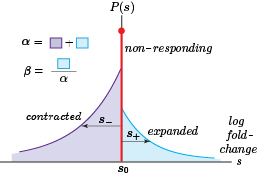
\includegraphics{schematic}
% \centering{}
% \caption{
% \emph{Functional forms of prior on clone size log-frequency fold-change}. $\rho(s)$,  \cref{eq:genPs}, is parametrized most generally here by an effect size for both expansion, $s_+$, and contraction,$s_-$, with an expanded fraction, $\beta$ of changed clones, the latter fraction of which itself a parameter, $\alpha$. Expansion and contraction is relative to the functions center, $s_0$, which can be fixed by the constraint $\langle f \rangle=\langle f^{\prime} \rangle$.
% \label{fig:Ps}}
% \end{figure}


%\begin{table}%[H] add [H] placement to break table across pages
%\caption{Prior functions used. See  \cref{fig:Ps} and  \cref{eq:genPs}. $\langle f \rangle= \langle f^{\prime} \rangle$ adds constraint, e.g. fixes $s_0$. \label{Tbl1:Priors}}
%\begin{ruledtabular}
%\begin{tabular}{c|c|c|c|c|c|c|c}
%index	& label				&$\alpha$ & $\beta$	& $s_-$    	& $s_+$		& $s_0$  & \#DOF ($s_0$ fixed) \\
%\hline
%0 		& $flat$ shift 	 	&$\alpha$ & $1/2$  	& $\infty$	& $\infty$  & $s_0$  & 2 \\
%1 		& $L=R$ 	 		&$\alpha$ & $1/2$  	& $\bar{s}$	& $\bar{s}$ & $0$    & 2 \\
%2 		& $L=R$ shift		&$\alpha$ & $1/2$  	& $\bar{s}$	& $\bar{s}$ & $s_0$  & 3(-1) \\
%3 		& $R$ only   		&$\alpha$ & $0$    	& n/a       & $\bar{s}$ & $0$    & 2 \\
%4 		& $R$ only shift  	&$\alpha$ & $0$  	& n/a       & $\bar{s}$ & $s_0$  & 3(-1) \\
%5 		& $L\neq R$  		&$\alpha$ & $\beta$	& $s_-$    	& $s_+$     & $0$    & 4 \\
%6 		& $L\neq R$ shift  	&$\alpha$ & $\beta$	& $s_-$    	& $s_+$     & $s_0$  & 5(-1)
%\end{tabular}
%\end{ruledtabular}
% \end{table}




\section*{Acknowledgements}
MPT would like to thank M. Pogorelly for providing the R code used to obtain the EdgeR estimates in \citep{Pogorelyy2018c}.  This work was supported by the European Research Council Consolidator Grant n. 724208.




\bibliographystyle{pnas}
\bibliography{thierry,diffexpr,max_response}

\newpage

%\section*{Appendices}


\beginsupplement


%\begin{figure}[ht!]
%%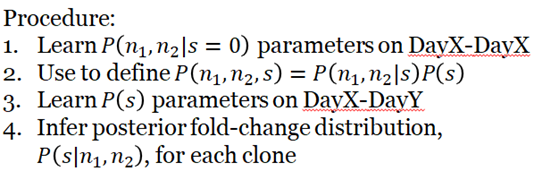
\includegraphics{procedure.png}
%%centering{}
%\caption{
%\emph{Supp. Fig: \re{What to show here?}Approximate equivalence of $N\langle f \rangle=1$ and $\mathcal{Z}^{\mathcal{D}}_f$.\label{fig:SM_match_null_constr}}}
%\end{figure}

\begin{figure}
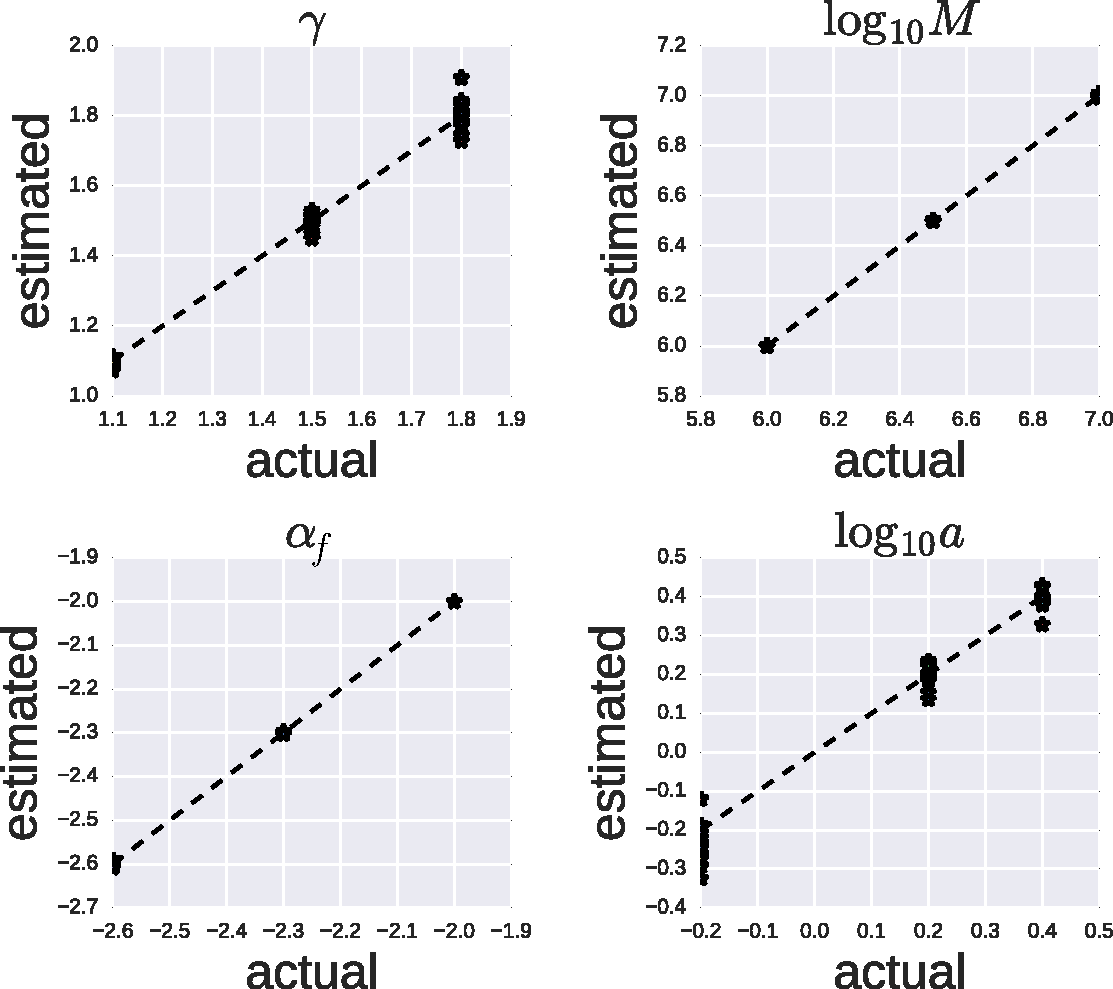
\includegraphics[width=\linewidth]{NB_Pois_nullpara_fits}
\centering{}
\caption{
\emph{Reinferring null model parameters}. Shown are the actual and estimated values of the null model parameters used to validate the null model inference procedure over the range exhibited by the data. A 3x3x3x3 grid of points were sampled and results collapsed over each parameter axis. $f_{\rm min}$ was fixed to satisfy the normalization constraint.
}
\label{fig:SM_reinfer_null}
\end{figure}

\begin{figure}
\includegraphics[width=\linewidth]{conditional_comparison}
\centering{}
\caption{
\emph{Dependence of conditional distribution $P(n^\prime=0|n)$ on $n$}. Two-step negative binomial to Poisson model captures tail better than one-step negative binomial model. Poisson model fits poorly. (Example donor S2-day 0 replicate pair.)\label{fig:SM_twostep_better}
}
\end{figure}



\begin{figure}
\includegraphics[width=\linewidth]{synthetic_reinference}
\centering{}
\caption{
\emph{Reinference of differential expression model for human-sized repertoire}. $10^9$ clones were sampled using $N_{\rm read}=10^6$ and $(\bar{s},\alpha)=(1.0,0.01)$ (cross), and clones with $n=n^\prime=0$ were removed. Note the orders of magnitude higher precision compared to the synthetic mouse repertoire \cref{fig:diffexpr_ex1}. 
\label{fig:SM_reinf_diffexpr}}
\end{figure}

\begin{figure}
\includegraphics[width=\linewidth]{s_naive_hist}
\centering{}
\caption{
\emph{Empirical histograms of naive log-frequency fold-change}. For example data: day-0/day-0 and day-0/day-15 pair comparisons averaged over donors.
\label{fig:SM_snaive_hists}
}
\end{figure}

\begin{figure}
\includegraphics[width=\linewidth]{s_med_vs_snaive}
\centering{}
\caption{
\emph{Summary statistics of log-frequency fold-change posterior distributions}. Comparison of the posterior median log-frequency fold-change and the naive estimate, $\log n^{\prime}/n$ (across clones with $n,n^{\prime}>0$). Each circle is a $(n,n^\prime)$ pair with size proportional to pair count average $(n+n^\prime)/2$ and intensity proportional to the number of observed clones with that pair.
\label{fig:SM_smed_snaive}
}
\end{figure}

\begin{figure}
\includegraphics[width=\linewidth]{posterior_ridge_sweep}

%\centering{}
\caption{
\emph{Competition between $\nu$ and $\bar{s}$ in shaping the posteriors, $\rho(s|0,n^\prime)$}. A) Posteriors for $n^\prime=9$ over a range of $(\bar{s},\alpha)$ pairs spanning the ridge shown in the inset in (B) and \cref{fig:volcano} along which the growth of $\bar{s}$ leads to $\rho(f)$ overwhelming $\rho_s(s)$ as the dominant explanation for observed expansion. (B) The posterior mean versus $\bar{s}$ for values of $n^\prime=1,\dots,9$, with the 5 values of $\bar{s}$ used in (A) shown for $n^\prime=9$.
\label{fig:posteriors}}
\end{figure}

\end{document}  












